\documentclass[../main.tex]{subfiles}

    \begin{document}
    \newpage

%%%%%%%%%%%%%%
    % Volet
    \vspace{15pt}
    %\needspace{20pt} % Réserve de l'espace
\section{Politique de sobriété foncière}

    % Block
\begin{block}[Maîtriser]
    \linespread{0.9}\selectfont % Réduit l'interligne
    \emoji{deciduous-tree} % Emoji
    \textit{\small{Encadrer l'artificialisation des sols pour préserver les ressources foncières.}}
\end{block}

    \begin{multicols}{2}
        \raggedcolumns
    \small{
\gras{Encadrer l’artificialisation des sols} constitue un impératif pour promouvoir un développement urbain soutenable. Une politique de sobriété des ressources foncières doit permettre \gras{d’optimiser l’usage des espaces déjà urbanisés} en orientant la croissance urbaine vers les territoires bien desservis, notamment au sein des quartiers de gare. Cela suppose la promotion d’un «~urbanisme circulaire~». En ce sens, nos travaux ont permis d’identifier finement les espaces à faible densité et bien connectés, présentant \gras{un potentiel de développement urbain}.
    \\\\
Cette politique doit prioriser \gras{le «~recyclage~» des friches}, \gras{la densification des tissus urbains} existants et \gras{la réhabilitation du bâti}, plutôt que l’extension urbaine. Une telle approche permet de limiter l’étalement non maîtrisé et de renforcer la résilience des territoires face aux îlots de chaleur. Dans les quartiers de gare, cette stratégie s’accompagne d’une gestion optimisée des espaces disponibles pour concilier les exigences d'accessibilité, d'usage des sols, de qualité de vie et de transition écologique.
    \\\\
Les objectifs du \gras{Zéro Artificialisation Nette (ZAN)} s'inscrivent pleinement dans cette démarche, qui visent à exploiter plus intelligemment ces espaces plutôt que d'ouvrir de nouvelles zones à l'urbanisation. L’intégration du vélo, de la micro-mobilité aux réseaux de transport en commun rend compatibles accessibilité et \gras{habitat individuel} à densité modérée.
    }
    %\\\\
\begin{center}
    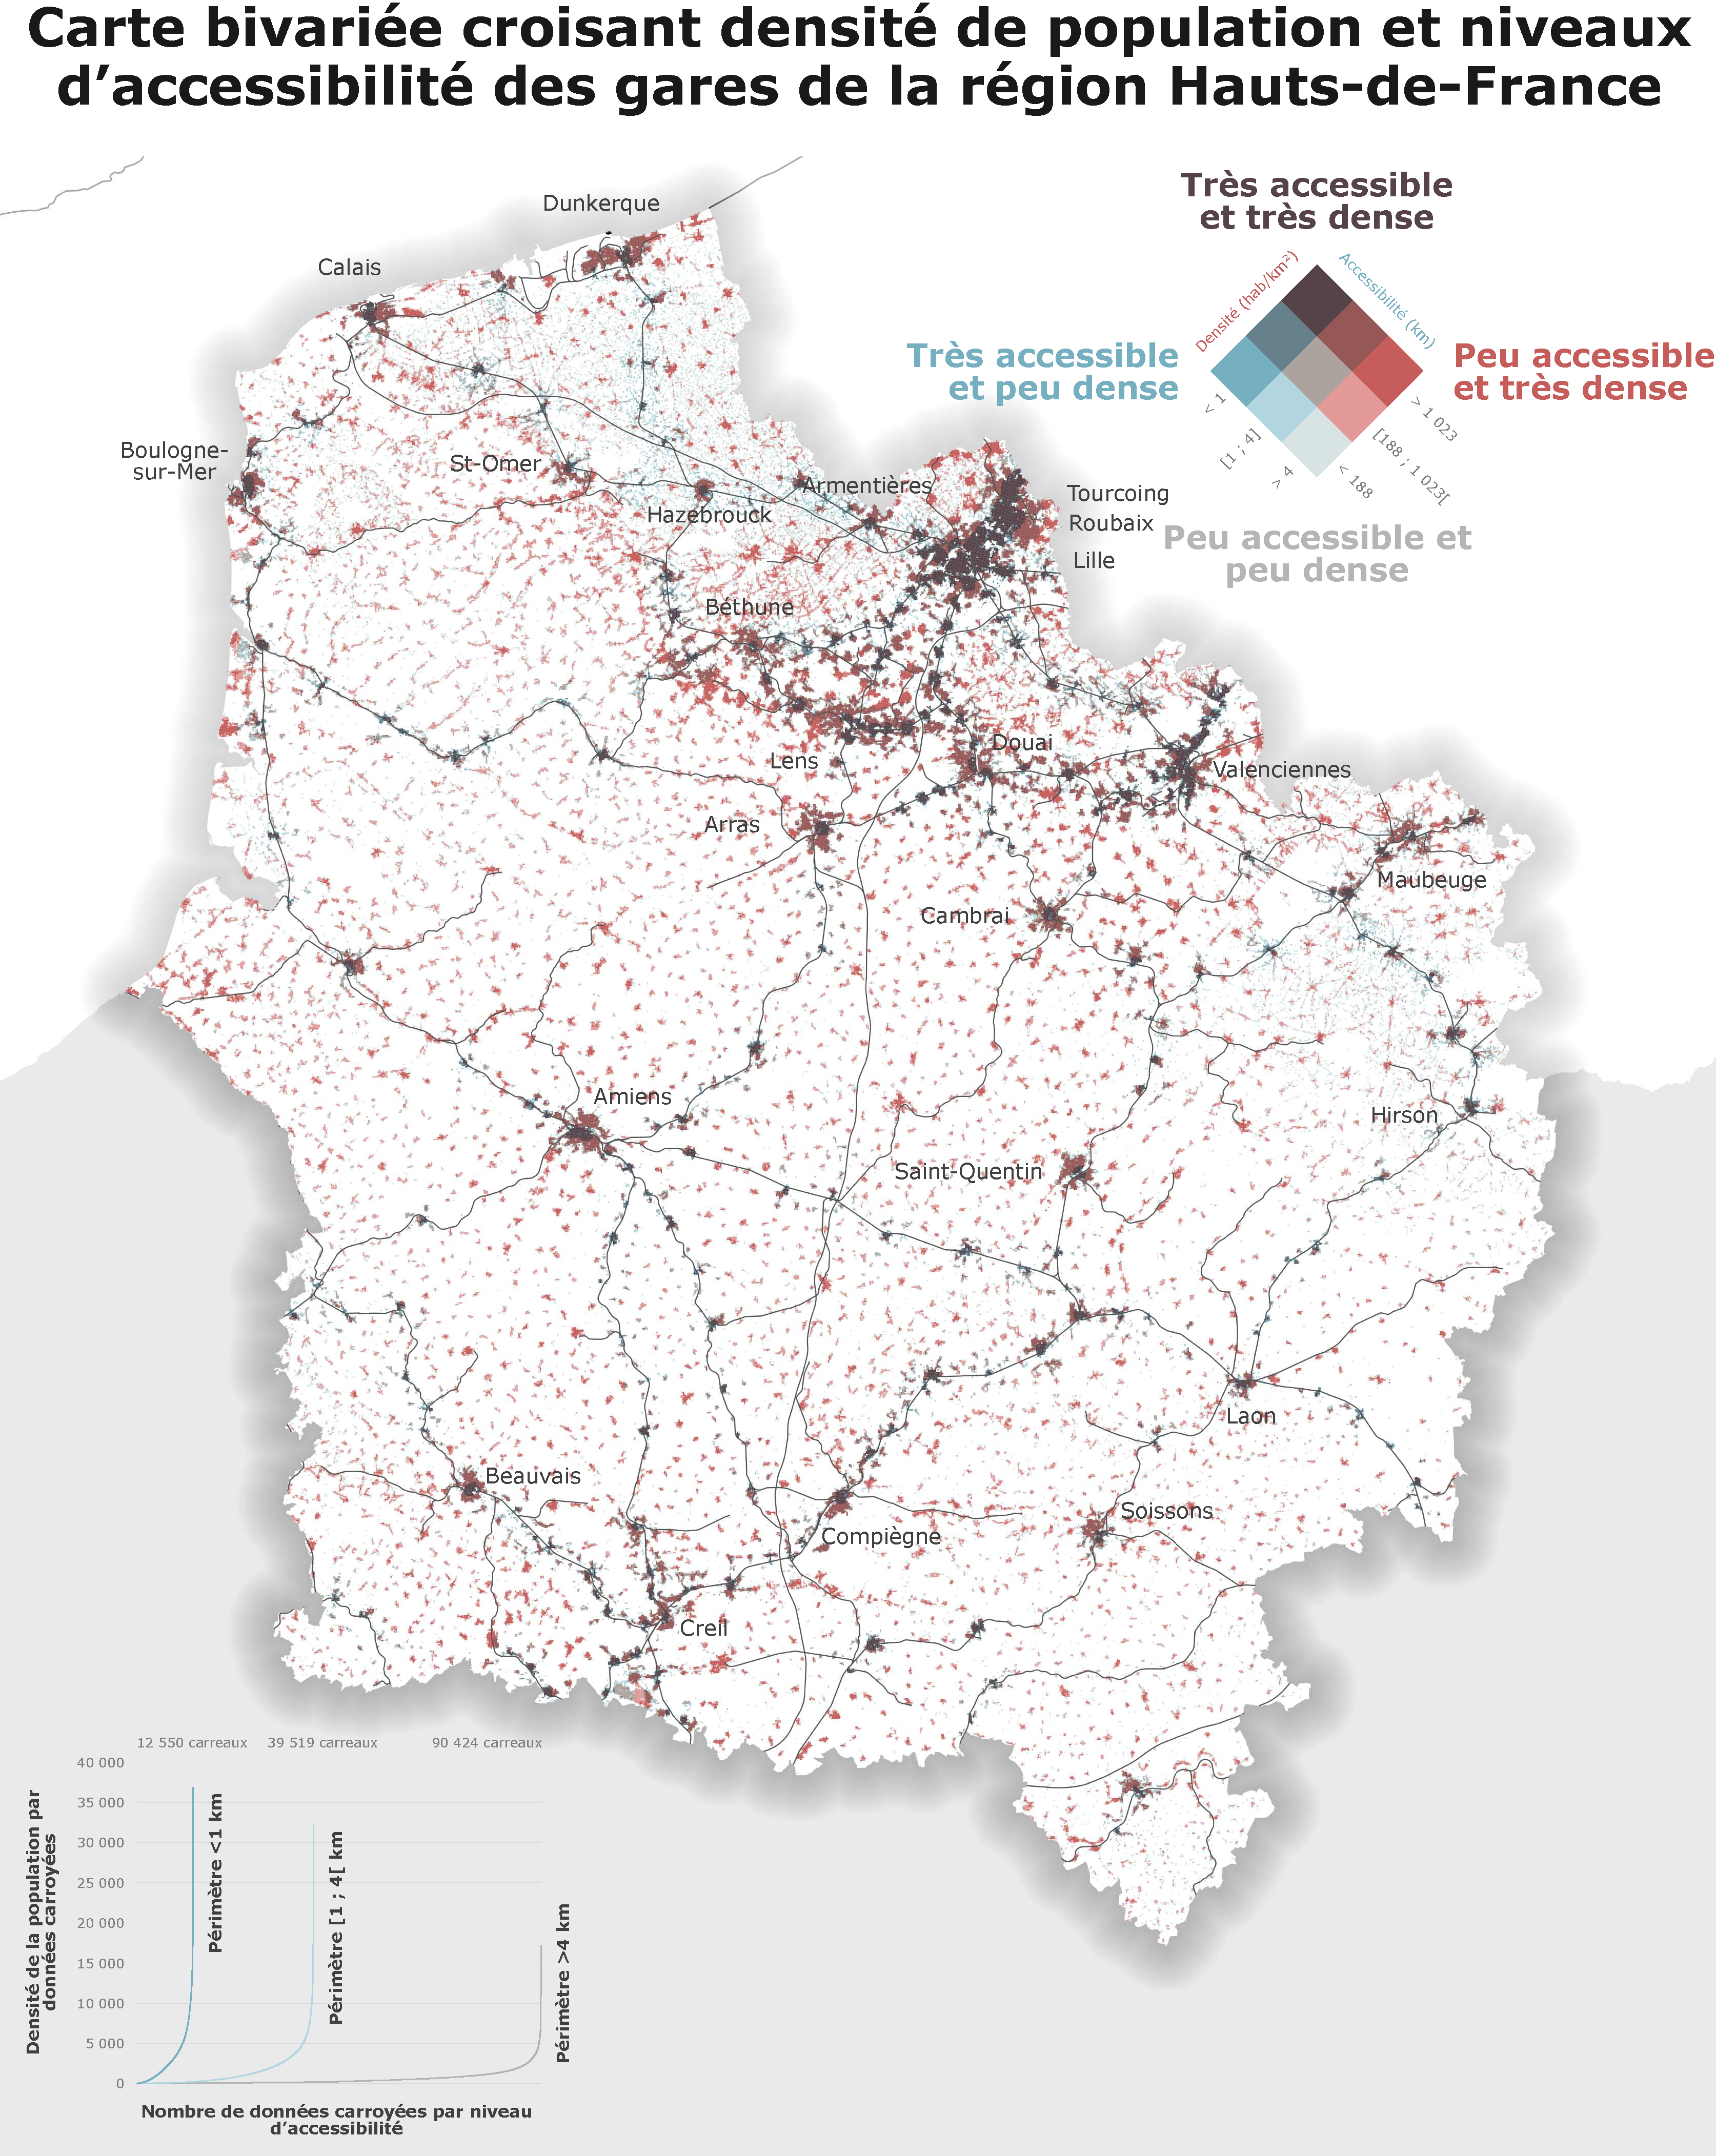
\includegraphics[width=\columnwidth]{figures/policy-brief-carte-densite-accessibilite-compresse.pdf}
    \label{densite-accessibilite}
    \vspace{-0.4cm}
    \begin{flushright}
            \scriptsize{\textcolor{darkgray}{Auteur~: Dylan Moinse (2025)}}
    \end{flushright}
\end{center}

    \end{multicols}

    \end{document}